\setcounter{chapter}{4}
\hyphenation{a-na-ly-ze}
\chapter{Statistical methods}\label{ch:stat}

\section{Introduction}

In the course of analyzing the data sets provided by the CMS experiment and used in this thesis, several statistical tools have been employed; in this chapter, a description of these tools will be presented, starting with the general statement of the multivariate analysis methods, followed by the particularities of the Boosted Decision Trees (BDT) method and its application to the classification problem. Statistical inference methods used will also be presented. This chapter is based mainly on References \cite{mva, tmva, luca}.      

\section{Multivariate analysis}\label{sec:mva}

Multivariate data analysis (MVA) makes use of the statistical techniques developed to analyze more than one variable at once, taking into account all the correlations among variables. MVA is employed in a variety of fields like consumer and market research, quality control and process optimization. Using MVA it is possible to identify the dominant patterns in a data sample, like groups, outliers and trends, and determine to which group a set of values belong; in the particle physics context, MVA methods are used to perform the selection of certain type of events from a large data set.

Processes with small cross section, such as the \tHq process ($\sigma_{SM}(\sqrt{s}=13 \textrm{TeV})=70.96$ fb), are hard to detect in the presence of the processes with larger cross sections, $\sigma_{SM}^{\ttbar}(\sqrt{s}=13 \textrm{TeV})=823.44$ fb for instance; therefore, only a small fraction of the data contains events of interest (signal), the major part is signal-like events, which mimic signal characteristics but belong to different processes, so they are a background to the process of interest. This implies that it is not possible to say with certainty that a given event is a signal or a background and statistical methods should be involved. In that sense, the challenge can be formulated as one where a set of events have to be classified according to certain special features; these features correspond to the measurements of several parameters like energy or momentum, organized in a set of \textit{input variables}. The measurements for each event can be written in a vector $\textbf{x}=(x_1,.....,x_n)$ for which

\begin{itemize}
\item $f(\textbf{x}|s)$ is the probability density (\ti{likelihood function}) that $\textbf{x}$ is the set of measured values given that the event is a signal event (signal hypothesis). 
\item $f(\textbf{x}|b)$ is the probability density (\ti{likelihood function}) that $\textbf{x}$ is the set of measured values given that the event is a background event (background hypothesis).
\end{itemize}

Figure \ref{fig:scatter_plot} shows three ways to perform a classification of events for which measurements of two properties, \ie, two input variables $x_1$ and $x_2$, have been performed; blue circles represent signal events while red triangles represent background events. The classification on the left is \textit{cut-based} requiring $x_1<c_1$ and $x_2<c_2$; usually the cut values ($c_1$ and $c_2$) are chosen according to some knowledge about the event process. In the middle plot, the classification is performed using a linear function of the input variables, hence the boundary is a straight line, while in the right plot the the relationship between input variables is not linear thus the boundary is not linear either.          

\begin{figure}[!h]
  \centering
  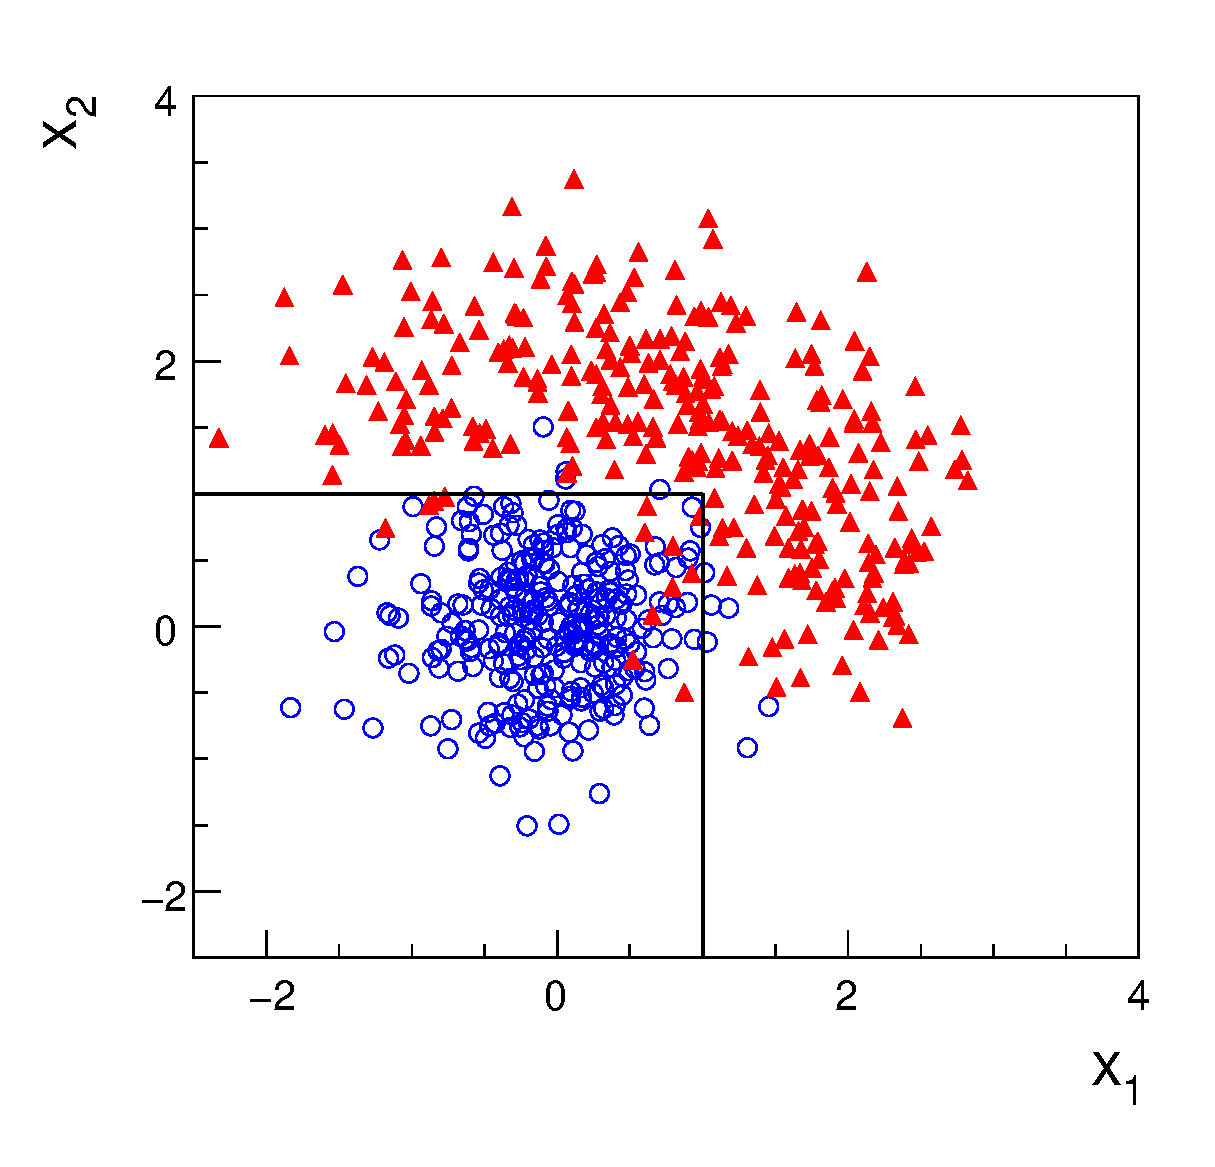
\includegraphics[width=4.5cm,height=4.5cm]{Cuts}
  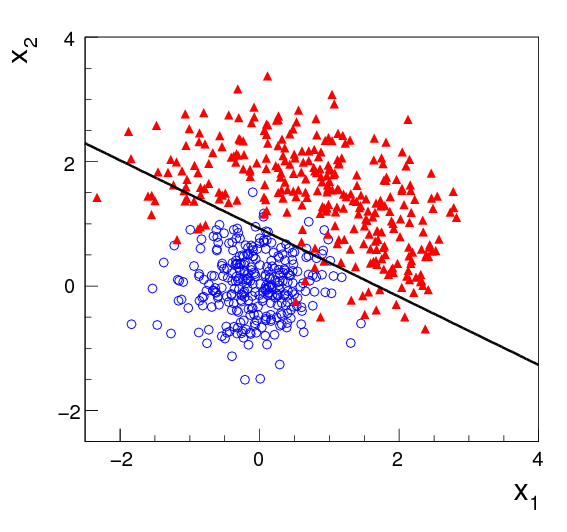
\includegraphics[width=4.5cm,height=4.5cm]{Fisher}
  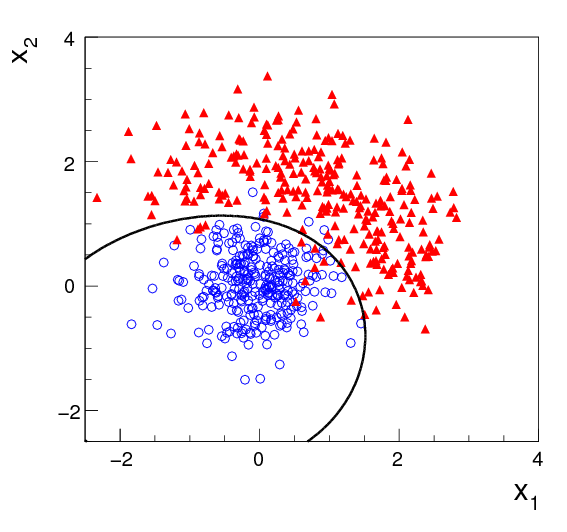
\includegraphics[width=4.5cm,height=4.5cm]{SVM05}
  \caption[Scatter plots-MVA event classification.]{Scatter plots-MVA event classification. Distribution of two input variables $x_1$ and $x_2$ measured for a set of events; blue circles represent signal events and red triangles represent background events. The classification is based on cuts (left), linear boundary (center), and nonlinear boundary (right)\cite{mva}}\label{fig:scatter_plot}.
\end{figure}

In general, the boundary can be parametrized in terms of the input variables such that the cut is set on the parametrization instead of on the variables, \ie, $y(\textbf{x})=y_{cut}$ with $y_{cut}$ being a constant; thus, the acceptance or rejection of an event is based on which side of the boundary the event is located. If $y(\textbf{x})$, usually called \ti{test statistic}, has functional form, it can be used to determine the probability distribution functions $p(y|s)$ and $p(y|b)$ and then perform a test statistic with a single cut on the scalar variable $y$. 

Figure \ref{fig:scalar_test} shows an example of what would be the probability distribution functions under the signal and background hypotheses for a scalar test statistic with a cut on the classifier $y$.
Note that the tails of the distributions indicate that some signal events fall in the rejection region and some background events fall on the acceptance region; therefore, it is convenient to define the \textit{efficiency} with which events of a given type are accepted. The signal and background efficiencies are given by 

\begin{figure}[!h]
  \centering
  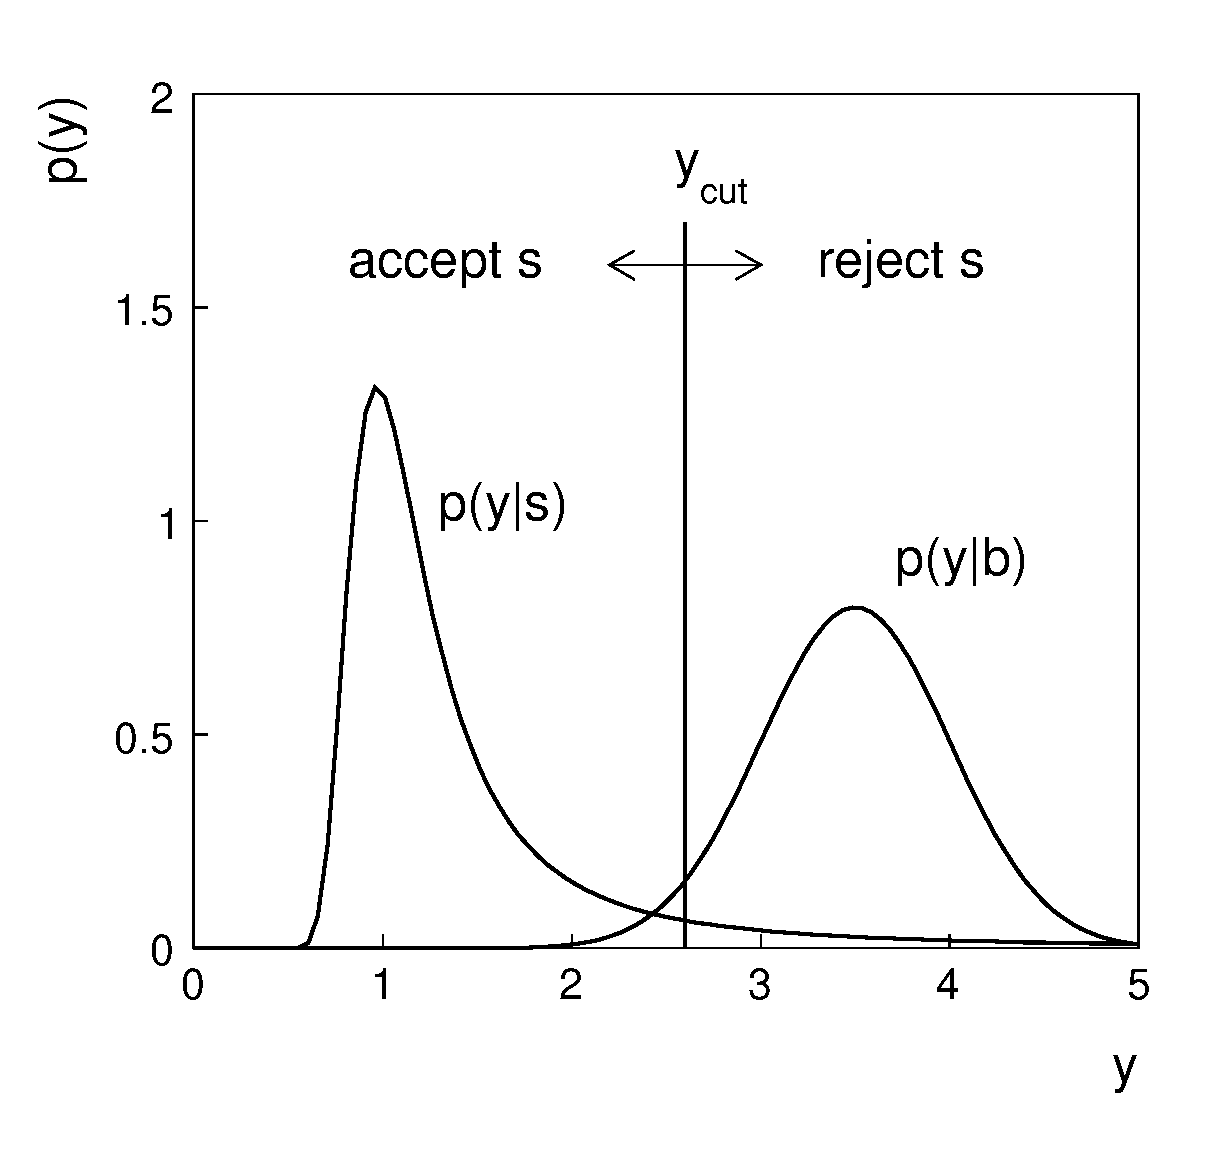
\includegraphics[scale=0.4]{TestStat}
  \caption[Scalar test statistical.]{Distributions of the scalar test statistic $y(\textbf{x})$ under the signal and background hypotheses.\cite{mva}}\label{fig:scalar_test}
\end{figure}

\begin{align}
\label{eq:sigeff}
\varepsilon_{\textrm{s}}  = & P( \mbox{accept event} | \mbox{s} ) = \int_{\textrm{A}} f(\textbf{x} | \mbox{s} ) \, d \textbf{x} = \int_{-\infty}^{y_{\textrm{cut}}} p(y | \mbox{s}) \, dy\;, \\
\varepsilon_{\textrm{b}}  = & P( \mbox{accept event} | \mbox{b} ) = \int_{\textrm{A}} f(\textbf{x} | \mbox{b} ) \, d \textbf{x} = \int_{-\infty}^{y_{\textrm{cut}}} p(y | \mbox{b}) \, dy \;,
\end{align}

\noindent where A is the acceptance region. If the background hypothesis is the \textit{null hypothesis ($H_0$)}, the signal hypothesis would be \textit{alternative hypothesis ($H_1$)}; in this context, the background efficiency corresponds to the significance level of the test ($\alpha$) and describes the misidentification probability, while the signal efficiency corresponds to the power of the test (1-$\beta$)\footnote{$\beta$ is the fraction of signal events that fall out of the acceptance region} and describes the probability of rejecting the background hypothesis if the signal hypothesis is true. What is sought in an analysis is to maximize the power of the test relative to the significance level, \ie, set a selection with the largest possible selection efficiency and the smallest possible misidentification probability.

\subsection{Decision trees}\label{subsec:dt}

For this thesis, the implementation of the MVA strategy, described above, is performed through decision trees by using the TMVA software package \cite{tmva} included in the ROOT analysis framework \cite{root}. In a simple picture, a decision tree classifies events according to their input variables values by setting a cut on each input variable and checking which events are on which side of the cut, just as proposed in the MVA strategy, but in addition, as a machine learning algorithm, decision trees offer the possibility to be trained and then perform the classification efficiently.   

\begin{figure}[!h]
  \centering
  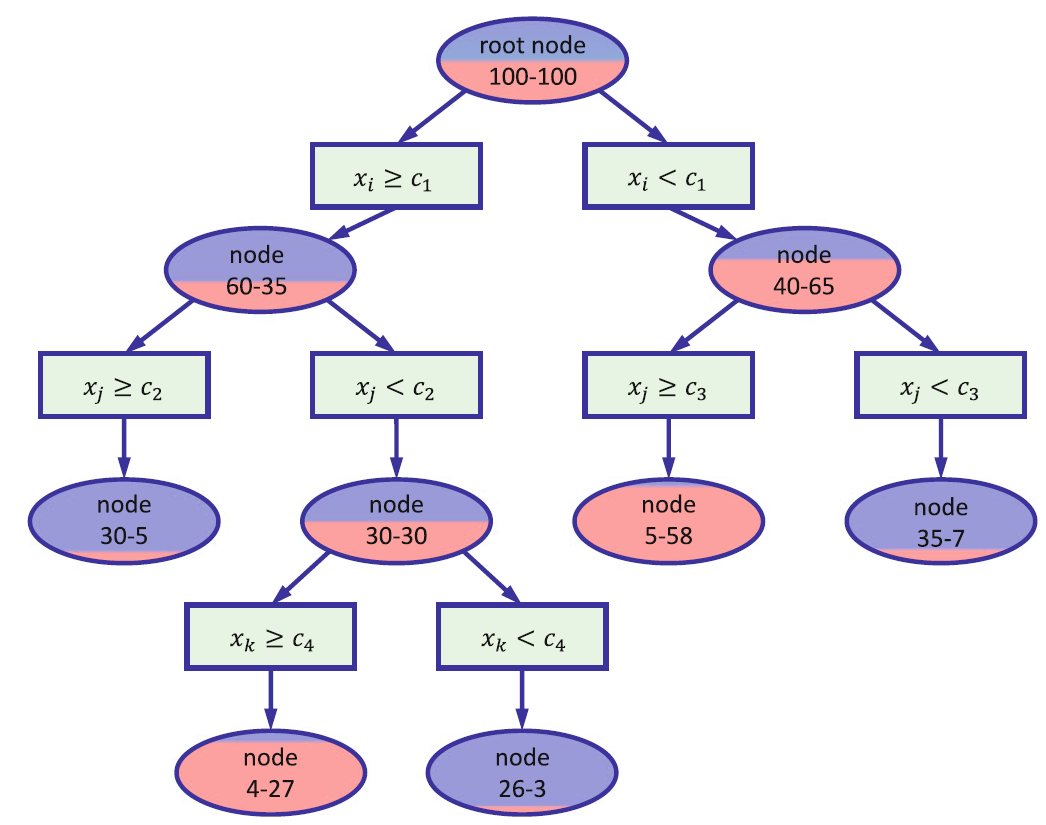
\includegraphics[scale=0.4]{decision_tree}
  \caption[Decision tree.]{Example of a decision tree. Each node is fed with a MC sample mixing signal and background events (left-right numbers); nodes colors represent the relative number of signal/background events \cite{luca}.}\label{fig:dt}
\end{figure}

The training or growing of a decision tree is the process where the rules for classifying events are defined; this process is represented in Figure \ref{fig:dt} and consists of several steps:

\begin{itemize}
\item take MC samples of signal and background events and split them into two parts each; the first parts will be used in the decision tree training, while the second parts will be used for testing the final classifier obtained from the training. Each event has associated a set of input variables $\textbf{x}=(x_1,.....,x_n)$ which serve to distinguish between signal and background events. The training sample is taken in at the \textit{root node}. 
\item Pick one variable, say $x_i$.
\item Pick one value of $x_i$, each event has its own value of $x_i$, and split the training sample into two subsamples $B_1$ and $B_2$; $B_1$ contains events for which $x_i< c_1$ while $B_2$ contains the rest of the training events;
\item scan all possible values of $x_i$ and find the splitting value that provides the \textit{best} classification\footnote{ Quality of the classification will be treated in the next paragraph.}, \ie, $B_1$ is mostly made of signal events while $B_2$ is mostly made of background events.
\item It is possible that variables other than the picked one produce a better classification, hence, all the variables have to be evaluated. Pick the next variable, say $x_j$, and repeat the scan over its possible values.
\item At the end, all the variables and their values will have been scanned, the \textit{best} variable and splitting value will have been identified, say $x_1, c_1$, and there will be two nodes fed with the subsamples $B_1$ and $B_2$. 
\end{itemize}

Nodes are further split by repeating the decision process until a given number of final nodes is obtained, nodes are largely dominated by either signal or background events, or nodes have too few events to continue. Final nodes are called \textit{leaves} and they are classified as signal or background leaves according to the class of the majority of events in them. Each \textit{branch} in the tree corresponds to a sequence of cuts. 

The quality of the classification at each node is evaluated through a separation criteria; there are several of them but the \textit{Gini Index (G)} is the one used in the decision trees trained for the analysis in this thesis. G is written in terms of the purity (P), \ie, the fraction of signal events in the samples after the separation is made; it is given by
\beqn
G=P(1-P)
\eeqn
\noindent note that P=0.5 at the root node while G=0 for pure leaves. For a node $A$ split into two nodes $B_1$ and $B_2$ the G gain is
\beqn
\Delta G = G(A)- G(B_1)-G(B_2).
\eeqn

The \textit{best} classification corresponds to that for which the gain of G is maximized; hence, the scanning over all the variables in an event and their values is of great importance.

In order to provide a numerical output for the classification, events in a signal(background) leaf are assigned an score of 1(-1) each, defining in this way the decision tree \textit{classifier/weak learner} as

\[
f(\textbf{x}) = \left\{
\begin{array}{ll}
  1  &  \textbf{x} \quad \textrm{in signal region,}\\
  -1 &  \textbf{x} \quad \textrm{in background region.}
\end{array}
\right.
\]

Figure \ref{fig:dtr} shows an example of the classification of a sample of events, containing two variables, performed by a decision tree.

\begin{figure}[!h]
  \centering
  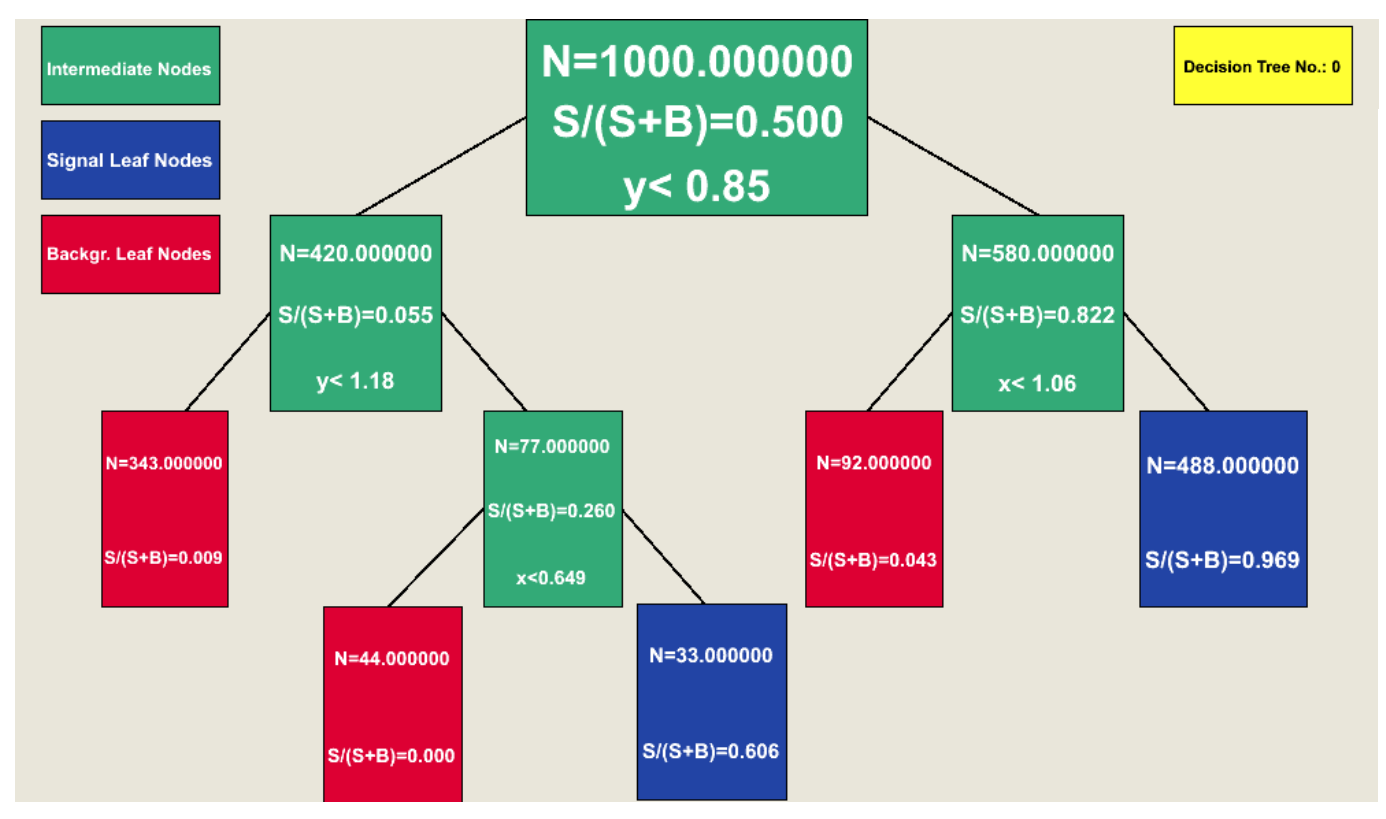
\includegraphics[scale=0.38]{dt1}
  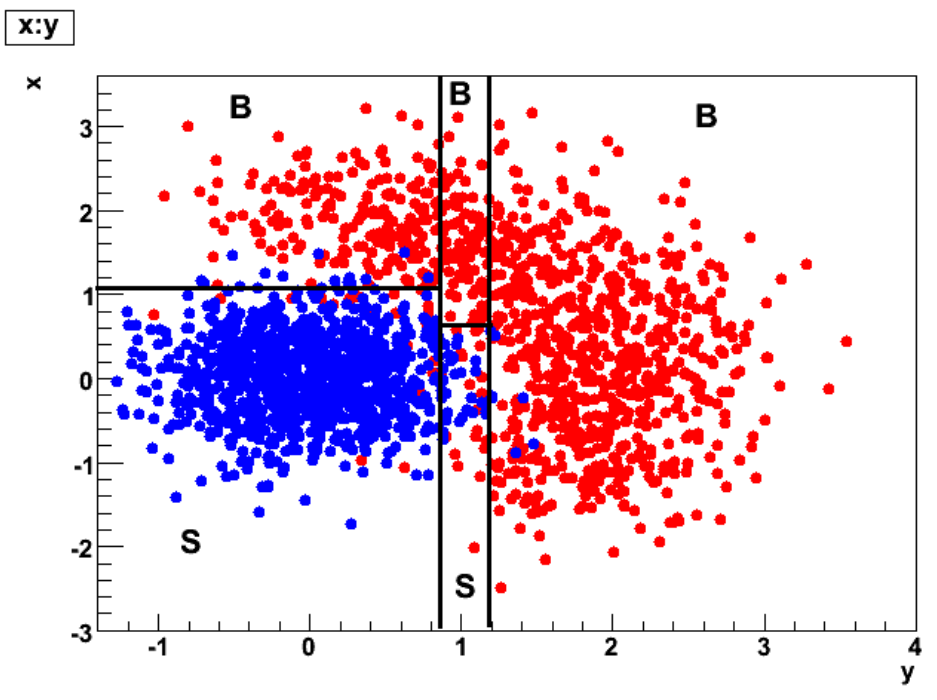
\includegraphics[scale=0.38]{dt2}
  \caption[Decision tree output example.]{Example of a decision tree output. Each leaf, blue for signal events and red for background events, is represented by a region in the variables phase space \cite{coadou}.}\label{fig:dtr}
\end{figure}

\subsection{Boosted decision trees (BDT).}

Event misclassification occurs when a training event ends up in the wrong leaf, \ie, a signal event ends up in a background leaf or a background event ends up in a signal leaf. A way to correct it is to assign a weight to the misclassified events and train a second tree using the reweighted events; the event reweighting is performed by a boosting algorithm in such a way that when used in the training of a new decision tree the \textit{boosted events} get correctly classified. The process is repeated iteratively adding a new tree to the forest and creating a set of classifiers, which are combined to create the next classifier; the final classifier offers more stability\footnote{Decision trees suffer from sensitivity to statistical fluctuations in the training sample which may lead to very different results with an small change in the training samples.} and has a smaller misclassification rate than any individual ones. The resulting tree collection is known as a \textit{boosted decision tree (BDT)}.

Thus, purity of the sample is generalized to 

\beqn
P=\frac{\sum_s w_s}{\sum_s w_s + \sum_b w_b}
\eeqn

\noindent where $w_s$ and $w_b$ are the weights of the signal and background events respectively; the Gini index is also generalized

\beqn
G=\left(\sum_i^n w_i\right) P(1-P)
\eeqn

\noindent with n the number of events in the node. The final score of an event, after passing through the forest, is calculated as the renormalized sum of all the individual (possibly weighted) scores; thus, high(low) score implies that the event is most likely signal(background).   

The boosting procedure, implemented in the  \textit{Gradient boosting} algorithm used in this thesis, produces a classifier $F(\textbf{x})$ which is the weighted sum of the individual classifiers obtained after each iteration, \ie,   

\beqn
F(\textbf{x})=\sum_{m=1}^M \beta_m f(\textbf{x};a_m)
\eeqn

\noindent where M is the number of trees in the forest. The \textit{loss function $L(F,y)$} represents the deviation between the classifier $F(\textbf{x})$ response and the true value $y$ obtained from the training sample (1 for signal events and -1 for background event), according to 

\beqn
L(F,y)= \textrm{ln}(1+ e^{-2F(\textbf{x})y})
\eeqn

\noindent thus, the reweighting is employed to ensure the minimization of the loss function; a more detailed description of the minimization procedure can be found in Reference \cite{friedman}. The final classifier output is later used as a final discrimination variable, labeled as \ti{BDT output/response}.

\subsection{Overtraining}

Decision trees offer the possibility to have as many nodes as desired in order to reduce the misclassification to zero (in theory); however, when a classifier is too much adjusted to a particular training sample, the classifier's response to a slightly different sample may leads to a completely different classification results; this effect is know as \ti{overtraining}.

An alternative to reduce the overtraining in BDTs consists in prunning the tree by removing statistically insignificant nodes after the tree growing is completed but this option is not available for BDTs with gradient boosting in the TMVA-toolkit, therefore, the overtraining has to be reduced by tuning the algorithm, number of nodes, minimum number of events in the leaves, etc. The overtraining can be evaluated by comparing the responses of the classifier when running over the training and test samples.   

\subsection{Variable ranking}

BDTs have a couple of particular advantages related to the input variables; they are relatively insensitive to the number of input variables used in the vector \textbf{x}. The ranking of the BDT input variables is determined by counting the number of times a variable is used to split decision tree nodes; in addition, the separation gain-squared achieved in the splitting and the number of events in the node are accounted by applying a weighting to that number. Thus, those variables with small or no power to separate signal and background events are rarely chosen to split the nodes, \ie, are effectively ignored.

In addition, variables correlations play an important role for some MVA methods like the Fisher discriminant algorithm in which the first step consist of performing a linear transformation to a phase space where the correlations between variables are removed; in the case of BDT algorithm, correlations do not affect the performance.

\subsection{BDT output example}

\begin{figure}[!h]
  \centering
  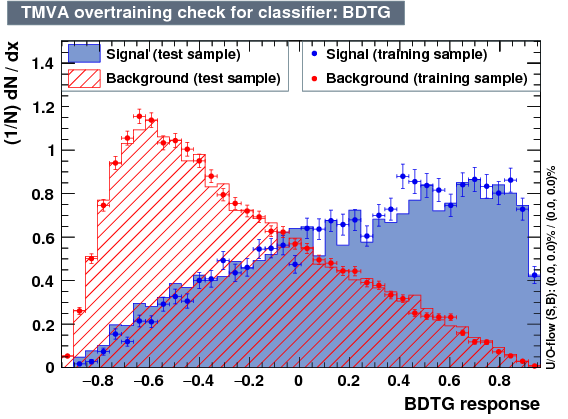
\includegraphics[scale=0.5]{bdt_output}
  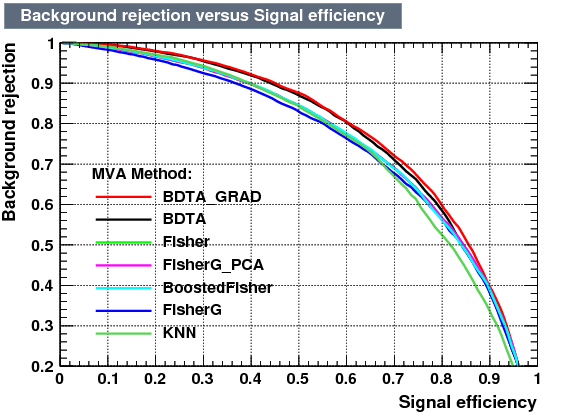
\includegraphics[scale=0.5]{roc_multimva}
  \caption[BDT output example.]{Left: Output distributions for the gradient boosted decision tree (BDTG) classifier using a sample of signal (\pp $\to$ \tHq) and background (\pp $\to$ \ttbar) events. Right: Background rejection vs signal efficiency (ROC curves) for various MVA classifiers running over the same sample used to produce the plot on the left.}\label{fig:bdt_output}
\end{figure}

The left side of figure \ref{fig:bdt_output} shows the BDT output distributions for signal (\pp $\to$ \tHq) and background (\pp $\to$ \ttbar) events; this plot is the equivalent to the one showed in Figure \ref{fig:scalar_test}. A forest with 800 trees, maximum depth per tree = 3, and gradient boosting have been used as training parameters. The BDTG classifier offers a good separation power. There is a small overtraining in the signal distribution, while the background distribution is very well predicted which might indicate that the sample is composed of more background than signal events.

The right side of figure \ref{fig:bdt_output} shows the background rejection vs signal efficiency curves for several combinations of MVA classifiers-boosting algorithms running over the same MC sample; these curves are known as ROC curves and give an indication of the performance of the classifier. In this particular example, the best performance is achieved with the BDTG classifier (BDTA\_GRAD), which motivate its use in this thesis.         

\section{Statistical inference}

Once events are classified, the next step consists of finding the parameters that define the likelihood functions $f(\textbf{x}|s), f(\textbf{x}|b)$ for signal and background events respectively. In general, likelihood functions depend not only on the measurements but also on parameters ($\theta_m$) that define their shapes; the process of estimating these \ti{unknown parameters} and their uncertainties from the experimental data is called \ti{inference}.     

The statistical inference tools used in this analysis are implemented in the RooFit toolkit \cite {roofit} and COMBINE package \cite{combine} included in the CMSSW software framework. 

\subsection{Nuisance parameters}

The unknown parameter vector $\bm{\theta}$ is made of two types of parameters: those parameters that provide information about the physical observables of interest for the experiment or \ti{parameters of interest}, and the \ti{nuisance parameters} that are not of a direct interest for the experiment but that need to be included in the analysis in order to achieve a satisfactory description of the data; they represent effects of the detector response like the finite resolutions of the detection systems, miscalibrations, and in general any source of uncertainty introduced in the analysis.

Nuisance parameters can be estimated from experimental data; for instance, data samples from a test beam are usually employed for calibration purposes. In cases where experimental samples are not availables, the estimation of nuisance parameters makes use of dedicated simulation programs to provide the required samples.

The estimation of the unknown parameters involves certain deviations from their true values, hence, the measurement of the nuisance parameter is written in terms of an estimated value, also called central value,  $\hat{\theta}$ and its uncertainty $\delta \theta$ using the notation

\beqn
\theta=\hat{\theta}\pm\delta \theta  
\eeqn

\noindent where the interval $[\hat{\theta}-\delta \theta, \hat{\theta}+\delta \theta]$ is called \ti{confidence interval}; it is usually interpreted, in the limit of infinite number of experiments, as the interval where the true value of the unknown parameter $\theta$ is contained with a probability of 0.6827 (if no other convention is stated); this interval represents the area under a Gaussian distribution in the interval $\pm 1\sigma$.    

Conventionally, uncertainties are split into two classes: \ti{systematic}, associated with the systematic effects, and \ti{statistical}, related only to fluctuations in data and having statistical nature. 

\subsection{Maximum likelihood estimation method}

The estimation of the unknown parameters that are in best agreement with the observed data is performed through a function of the data sample that returns the estimate of those parameters; that function is called an \ti{estimator}. Estimators are usually constructed using mathematical expressions encoded in computer programs. 

In this thesis, the estimator used is the likelihood function $f(\textbf{x}|\bm{\theta})$\footnote{analogue to the likelihood functions described in previous sections} which depends on a set of measured variables $\textbf{x}$ and a set of unknown parameters $\bm{\theta}$. The likelihood function for N events in a sample is the combination of all the individual likelihood functions, \ie, 

\beqn
L(\bm{\theta})=\prod_{i=1}^N f(\textbf{x}^i|\bm{\theta})=\prod_{i=1}^N f(x^i_1,...,x_n^i;\theta_1,...,\theta_m)\label{eqn:ml}
\eeqn

\noindent and the estimation method used is the \ti{Maximum Likelihood Estimation} method (MLE); it is based on the combined likelihood function defined by eqn. \ref{eqn:ml} and the procedure seeks for the parameter set that corresponds to the maximum value of the combined likelihood function, \ie, the \ti{maximum likelihood estimator} of the unknown parameter vector $\bm{\theta}$ is the function that produces the vector of \ti{best estimators} $\bm{\hat \theta}$ for which the likelihood function $L(\bm{\theta})$ evaluated at the measured $\textbf{x}$ is maximum.  

Usually, the logarithm of the likelihood function is used in numerical algorithm implementations in order to avoid underflow the numerical precision of the computers due to the product of small likelihoods. In addition, it is common to minimize the negative logarithm of the likelihood function, therefore, the negative log-likelihood function is
%instead of maximizing the logarithm of it because in this way the procedure consist of differentiate a sum of therms and setting the sum to zero;
\beqn
F(\bm{\theta}) = -\textrm{ln}L(\bm{\theta})=-\sum_{i=1}^N f(\textbf{x}^i|\bm{\theta}).
\eeqn

The minimization process is performed by the software MINUIT \cite{minuit} implemented in the ROOT analysis framework. In case of data samples with large number of measurements, the computational resources necessary to calculate the likelihood function are too big; therefore, the parameter estimation is performed using binned distributions of the variables of interest for which the \ti{binned likelihood function} is given by
\beqn
L(\textbf{x}|r,\bm{\theta})=\prod_{i=1} \frac{(r\cdot s_i(\bm{\theta})+ b_i(\bm{\theta}))^{n_i}}{n_i!} e^{-r\cdot s_i(\bm{\theta})-b_i(\bm{\theta})} \prod_{j=1}\frac{1}{\sqrt{2\pi}\sigma_{\theta_j}^2}e^{-(\theta_j-\theta_{0,j})^2/2\sigma_{\theta_j}^2} ,\label{eqn:bml}
\eeqn

\noindent with $s_i$ and $b_i$ the expected number of signal and background yields for the bin $i$, $n_i$ is the observed number of events in the bin $i$ and $r = \sigma/\sigma_{SM}$ is the signal strength. Note that the number of entries per bin follows a Poisson distribution. The effect of the nuisance parameters have been included in the likelihood function through Gaussian distributions that models the nuisance. The three parameters, r, $s_i$ and $b_i$ are jointly fitted to estimate the value of r.

%The analysis presented in this thesis is based on the binned distribution of the ratio signal/background obtained from the BDT outputs

\section{Upper limits }

In this analysis, two hypotheses are considered; the background only hypothesis ($H_0(b)$) and the signal plus background hypothesis ($H_1(s+b)$), \ie, the sample of events is composed of background only events (r=0) or it is a mixture of signal plus background events (r=1). The exclusion of one hypothesis against the other means that the observed data sample better agrees with $H_0$ or rather with $H_1$. In order to discriminate these hypotheses, a test statistic is constructed on the basis of the likelihood function evaluated for each of the hypothesis.  

The \ti{Neyman-Pearson} lemma \cite{npl} states that the test statistic that provides the maximum power for $H_1$ for a given significance level (background misidentification probability $\alpha$), is given by the ratio of the likelihood functions $L(\textbf{x}|H_1)$ and $L(\textbf{x}|H_0)$; however, in order to use that definition it is necessary to know the true likelihood functions, which in practice is not always possible. Approximate functions obtained by numerical methods, like the BDT method described above, have to be used, so that the \ti{profile likelihood} test statistic is defined by 

\beqn
\lambda(\textbf{r})=\frac{L(\textbf{x}|r,\hat{\hat{\bm{\theta}}}(r))}{L(\textbf{x}|\hat r, \hat{\bm{\theta}})},
\eeqn

\noindent where, $\hat r$ and $\hat{\bm{\theta}}$ maximize the likelihood function, and $\hat{\hat{\bm{\theta}}}$ maximizes the likelihood function for a given value of the signal strength modifier $r$. In practice, the test statistic $t_r$
\beqn
t_r=-2\textrm{ln} \lambda(r)  
\eeqn

\noindent is used to evaluate the presence of signal in the sample, since the minimum of $t_r$ at $r=\hat r$ suggests the presence of signal with signal strength $\hat r$. The uncertainty interval for $r$ is determined by the values of $r$ for which $t_r=+1$. 

\begin{figure}[!h]
  \centering
  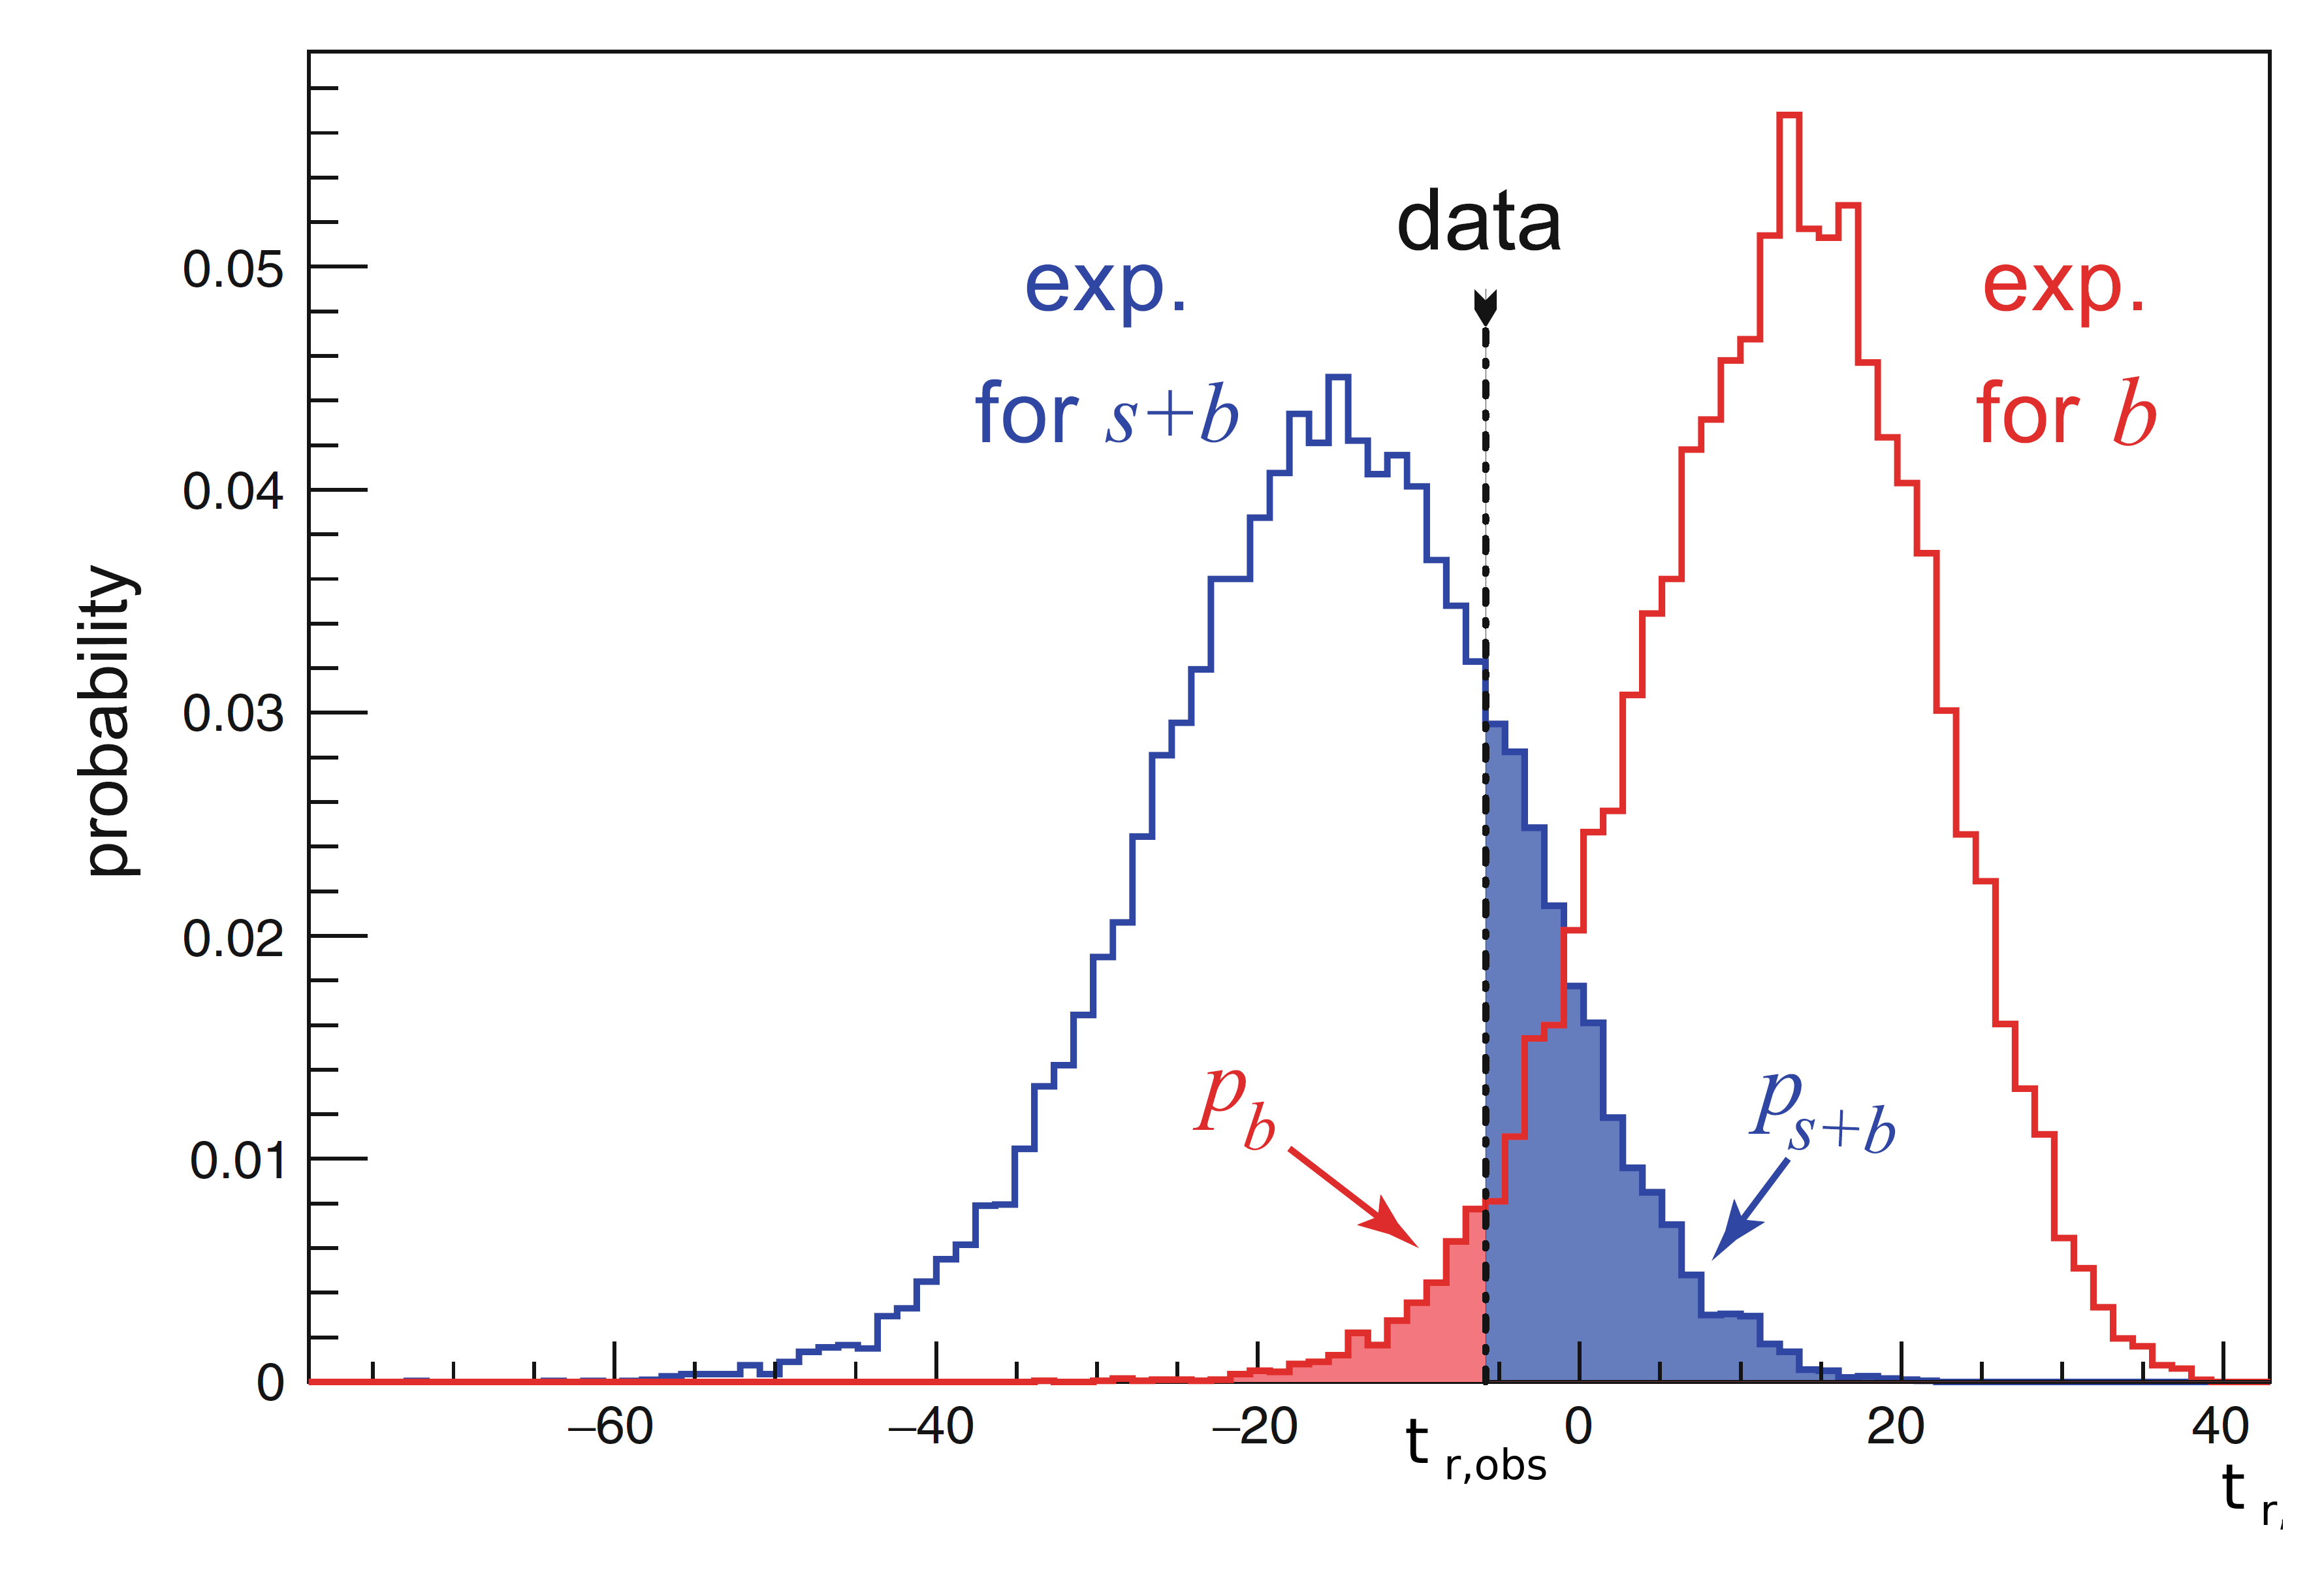
\includegraphics[width=0.8\textwidth]{t_r}
  \caption[$t_r$ p.d.f. assuming each $H_0$ and $H_1$]{ $t_r$ p.d.f. from MC pseudo experiments assuming $H_0$ (red) and $H_1$ (blue). The black dashed line shows the value of the test statistic as measured from data. Adapted from Reference \cite{luca}.}\label{fig:t_r}
\end{figure}


The expected probability density function (p.d.f) $f({t_r|r,\bm{\theta}})$ of the test statistic $t_r$ can be obtained numerically by generating MC samples where one hypothesis, $H_0(b)$ or $H_1(s+b)$, is assumed; thus, MC samples contain the possible values of $t_r$ obtained from \ti{pseudo-experiments} as shown in Figure \ref{fig:t_r}. The probability that $t_r$ takes a value equal or greater than the observed value ($t_{r,obs}$) when a signal with a signal modifier $r$ is present in the data sample, is called the \ti{p-value} of the observation; it can be calculated using 

\beqn
p_r=\int_{t_{r,obs}}^\infty f(t'_r|r, \bm{\theta}) dt'_r,
\eeqn

\noindent thus, $p_r < 0.05$ means that, for that particular value of $r$, $H_1$ could be excluded at 95\% Confidence Level (CL). The corresponding background-only p-value is given by

\begin{figure}[!h]
  \centering
  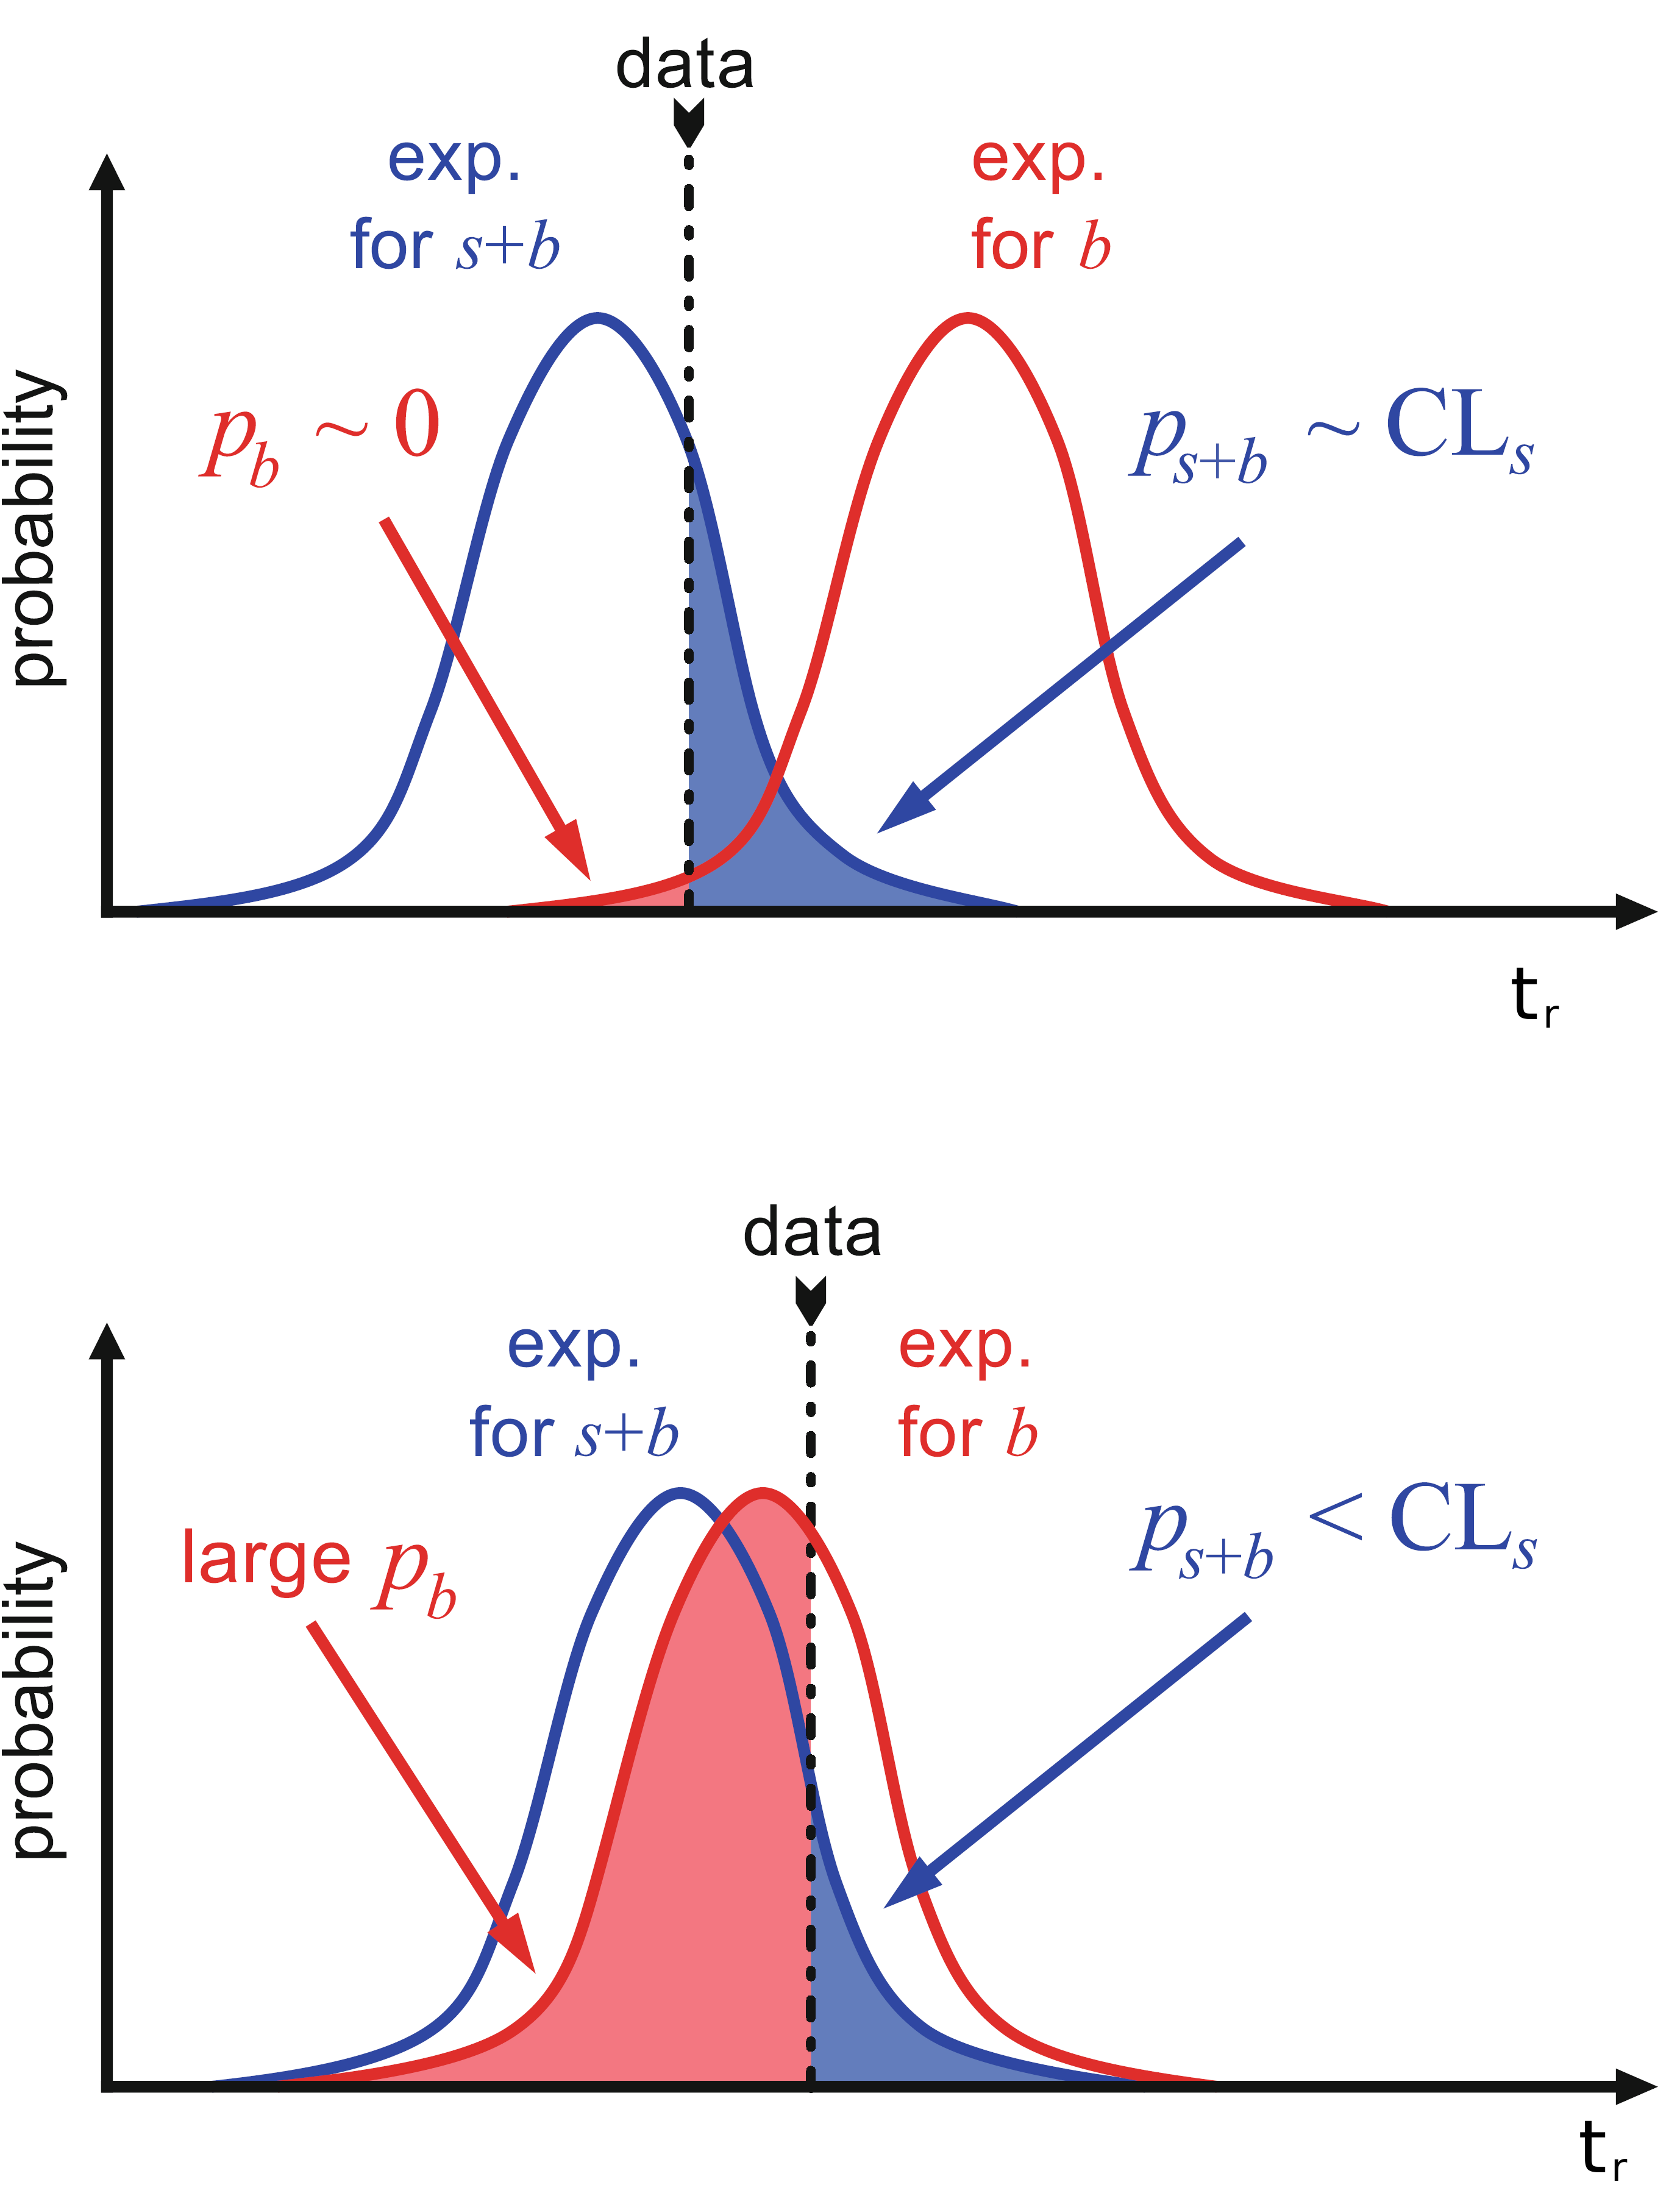
\includegraphics[width=0.6\textwidth]{t_r2}
  \caption[Illustration of the $CL_s$ limit.]{ $CL_s$ limit illustration. When the test statistic p.d.f. for the two hypotheses $H_0$ and $ H_1$ are well separated (top) and when they are largely overlapped (bottom). Adapted from Reference \cite{luca}.}\label{fig:t_r2}
\end{figure}

\beqn
1-p_b=\int_{t_{r,obs}}^\infty f(t'_r|0,\bm{\theta}) dt'_r,
\eeqn

If the $t_r$ p.d.f.s for both hypotheses are well separated, as shown in the top side of Figure \ref{fig:t_r2}, the experiment is sensitive to the presence of signal in the sample. If the signal presence is small, both p.d.f.s will be largely overlapped (bottom of Figure \ref{fig: t_r2}) and either the signal hypothesis could be rejected with not enough justification because the experiment is not sensitive to the signal or a fluctuation of the background could be misinterpreted as presence of signal with the corresponding rejection of the background-only hypothesis. These issues are corrected by using the modified p-value \cite{read}

\beqn
p'_r= \frac{p_r}{1-p_b} \equiv CL_s.\label{eqn:cls}
\eeqn

If $H_1$ is true, then $p_b$ is small, $CL_s\simeq p_r$ and $H_0$ is rejected; if there is large overlap and a statistical fluctuation causes that $p_b$ is large, then both numerator and denominator in Eqn. \ref{eqn:cls} become small but $CL_s$ would allow the rejection of $H_1$ even if there is poor sensitivity to signal.     

The upper limit of the parameter of interest $r^{up}$ is determined by excluding the range of values of $r$ for which $CL_s(r,\bm{\theta})$ is lower than the confidence level desired, normally 90\% or 95\%, e.g, scanning over $r$ and finding the value for which $p_r^{'up}=0.05$. The expected upper limit can be calculated using pseudo-experiments based on the background-only hypothesis and obtaining a distribution for $r^{up}_{ps}$; the median of that distribution corresponds to the expected upper limit, while the $\pm 1\sigma$ and $\pm2\sigma$ deviations correspond to the values of the distribution that defines the 68\% and 95\% of the area under the distribution centered in the median. It is usual to present all the information about the expected and observed limits in the so-called \ti{Brazilian-flag plot} as the one showed in Figure \ref{fig:hgg}. The solid line represent the observed $CL_s$  

\begin{figure}[!h]
  \centering
  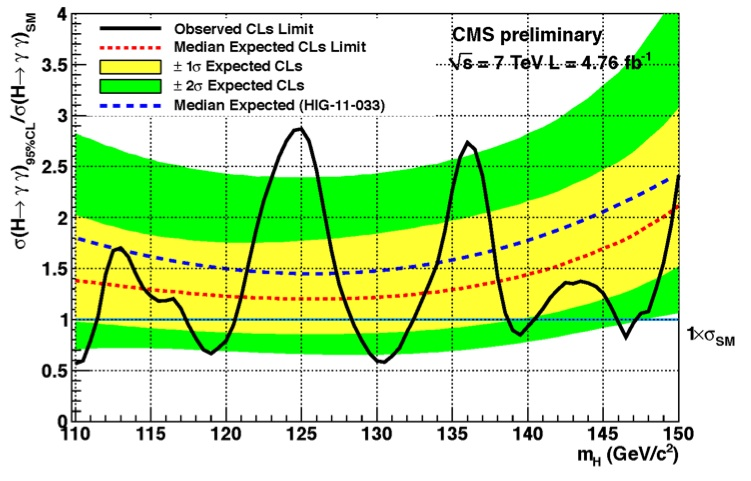
\includegraphics[width=0.6\textwidth]{Hgg}
  \caption[Example of Brazilian flag plot]{ Brazilian flag plot of CMS experiment limits for Higgs boson decaying to photons \cite{hgg}.}\label{fig:hgg}
\end{figure}

\section{Asymptotic limits}

As said before, the complexity of the likelihood functions, the construction of test statistics, and the calculation of the limits and their uncertainties is not always manageable and requires extensive computational resources; in order to overcome those issues, asymptotic approximations for likelihood-based test statistics, like the ones described in previous sections, have been developed \cite{wald,asymptotic} using Wilks' theorem. Asymptotic approximations replace the construction of the test statistics p.d.f.s using MC pseudo-experiments, with the approximate calculation of the test statistics p.d.f.s by employing the so-called \ti{Asimov dataset}.

The Asimov dataset is defined as the dataset that produce the true values of the nuisance parameters when it is used to evaluate the estimators for all the parameters; it is obtained by setting the values of the variables in the dataset to their expected values \cite{asymptotic}.

Limits calculated by using the asymptotic approximation and the Asimov dataset are know as \ti{asymptotic limits}.
